\setchapterpreamble[u]{\margintoc}
\chapter{Transformada de Legendre}
\labch{Legendre}


La transición del lagrangiano y $\mathbf{T Q}$ al hamiltoniano y $\mathbf{T}^{*} \mathbb{Q}$ es un ejemplo de lo que se denomina transformación de Legendre. Explicamos esto en una dimensión y luego indicamos cómo extender la explicación a más de una.

Consideremos una función diferenciable $L(v)$ de una sola variable $v$. Para cada valor de $v$ en su dominio, la función da el número $L(v)$ en su intervalo, y su gráfica es la curva continua de todos los puntos (v, $L(v)$ ) (Fig. 5.1). En cada punto la función tiene una derivada (la curva tiene una tangente), que escribimos

\begin{marginfigure}[]
  
  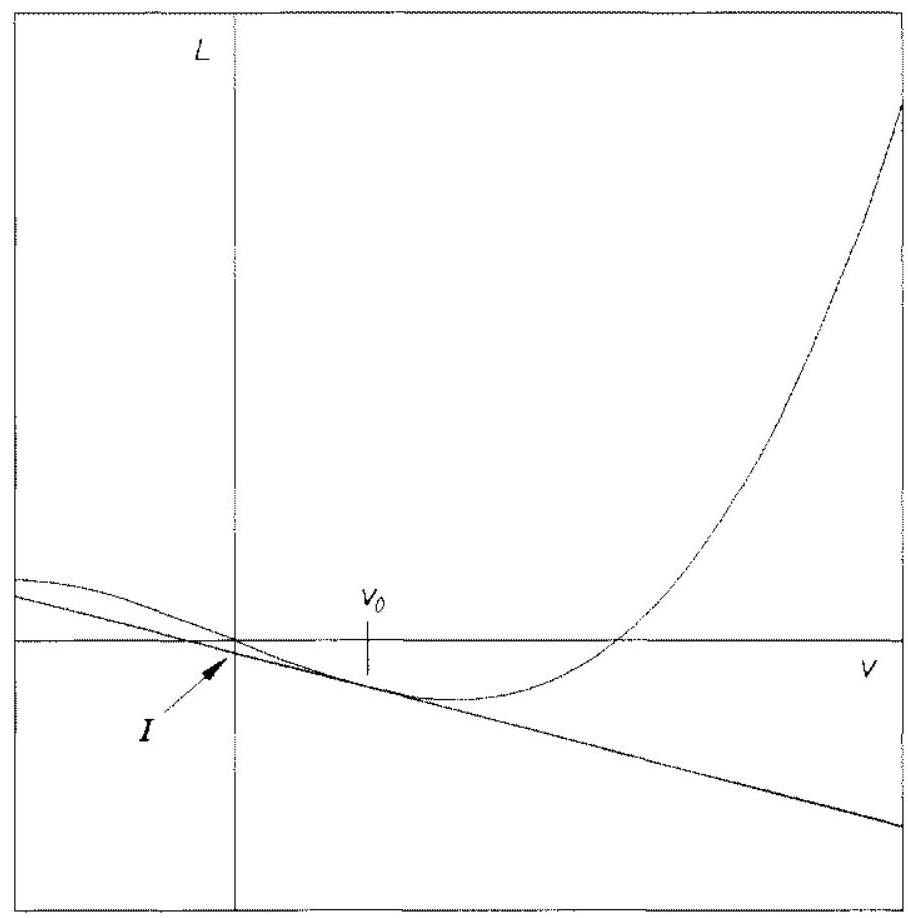
\includegraphics{Legen1.jpg}
  \caption[]{Una función $L(v)$, que tiene un punto de inflexión en el origen. La tangente a la curva en $v=v_{0}$ tiene pendiente $p=d L / d v$ calculada en $v_{0}$. La intersección en el eje $L$ se denomina $I$.}
  \labfig{fig:}
\end{marginfigure}

\begin{equation*}
  p(v) \equiv d L(v) / d v \tag{5.36}
\end{equation*}

\begin{definition}[Transformada de Legendre]
  La transformada de Legendre es una forma de describir la función o reproducir la gráfica enteramente en términos de $p$, sin referencia a $v$ : es decir, $p$ se convertirá en la variable independiente cuyos valores se utilizan para construir la curva. Pero del mismo modo que los valores de $v$ por sí solos, sin los valores de $L(v)$, no bastan para definir la curva, los valores de $p$ por sí solos tampoco bastan. Lo que se necesita es una función $H(p)$ de la nueva variable $p$.
\end{definition}


La función $H(p)$ se obtiene de la siguiente manera. Partimos de la Fig. 5.1, que muestra la tangente a la curva $L(v)$ en el punto $v=v_{0}$. La pendiente de esta tangente es $p\left(v_{0}\right) \equiv p_{0}$, y su intersección $I$ en el eje $L$ viene dado por

\[I=L\left(v_{0}\right)-p_{0} v_{0}\]

Hay una intersección diferente para cada $v$ en la curva (entonces eliminamos el subíndice 0 ), por lo que el intercepto se convierte en una función del punto $v$ y de la derivada $p$ en ese punto:
\begin{equation*}
  I(v, p)=L(v)-p v \tag{5.37}
  \end{equation*}

  Supongamos ahora que la Ec. (5.36) es invertible, de modo que $v$ puede obtenerse como función de $p$. En ese caso cada valor de $p$ determina unívocamente un valor de $v$ : una pendiente dada se da sólo en un punto de la curva. (La función de la Fig. 5.1 no cumple este requisito: la misma pendiente se da en más de un punto. Volveremos sobre esto más adelante). Cuando se encuentra $v(p)$, se puede sustituir por $v$ en (5.37), que se convierte entonces en una función de $p$ solamente. Entonces $H(p)$ se define por

  Hasta ahora $H(p)$ se ha obtenido a partir de $L(v)$. Ahora demostraremos que $L(v)$ puede obtenerse a partir de $H(p)$, y por tanto que las dos funciones son equivalentes. Primero lo demostraremos gráficamente y luego analíticamente.

  \begin{marginfigure}[]
    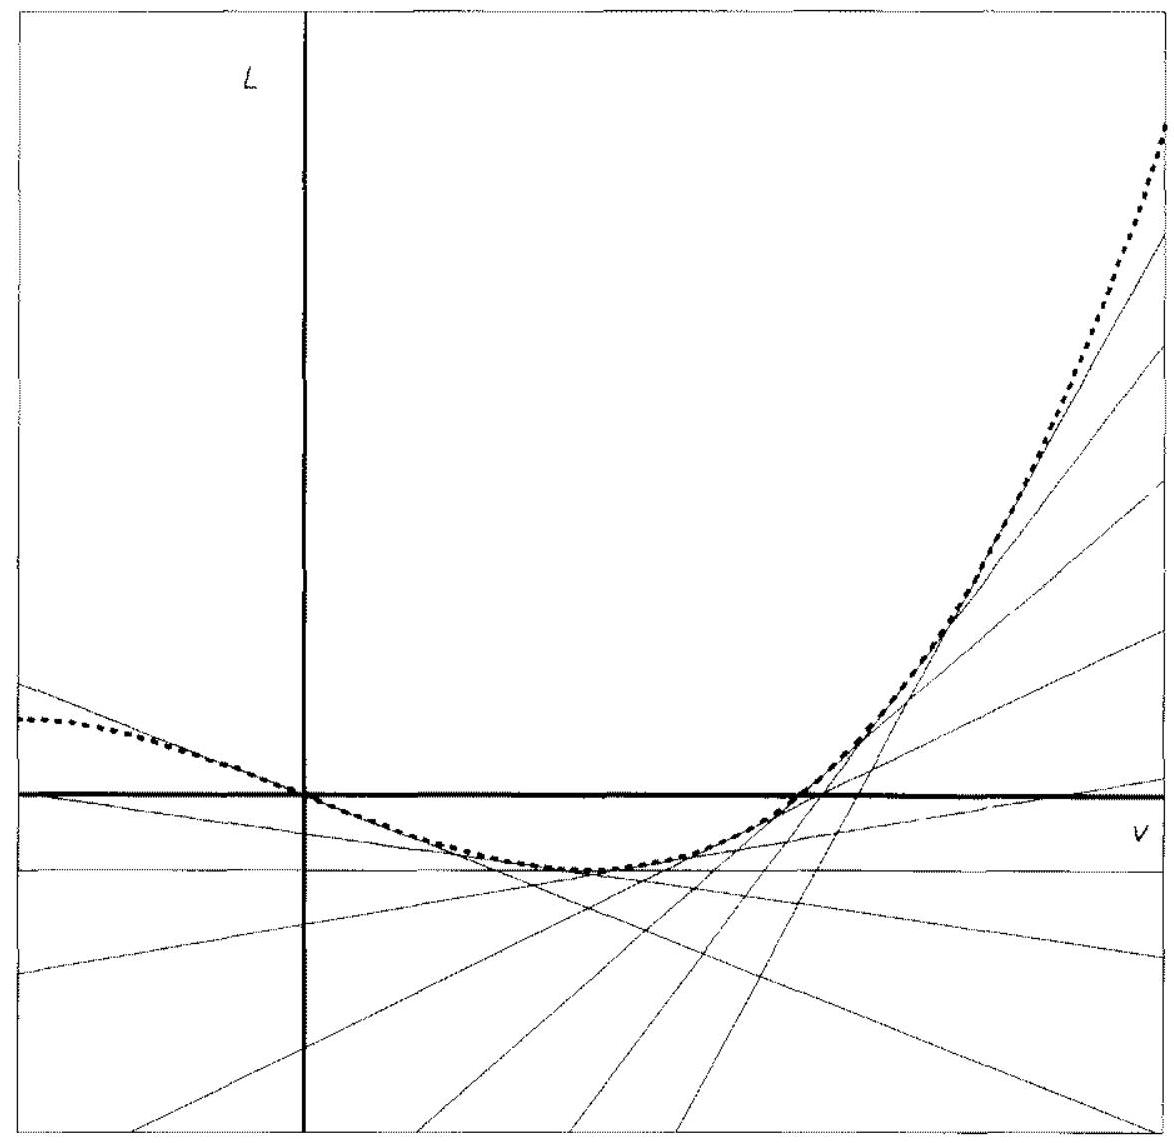
\includegraphics{Legen2.jpg}
    \caption[]{Tangentes a la curva $L(v)$ de la Fig. 5.1 para valores de $v$ por encima del punto de inflexión, obtenidas calculando ( $p, H(p)$ ) para varios valores de $p$. La curva punteada es $L(v)$, vista como la envolvente de las tangentes.}
    \labfig{fig:}
  \end{marginfigure}


  Supongamos que se conoce $H(p)$. Cada combinación $(p, H(p))$ corresponde a una recta de pendiente $p$ e intercepto $-H(p)$ sobre el eje $L$ en el plano $(L, v)$. El conjunto de tales rectas para $v>0$ (donde la relación entre $v$ y $p$ es única) en la Fig. 5.1 se muestra en la Fig. 5.2. La curva $L(v)$ es la envolvente de estas rectas, la curva continua tangente a todas ellas. Así pues, la curva $L(v)$ (o parte de ella) se ha construido a partir de $H(p)$.

  La prueba analítica requiere demostrar que la función $L(v)$ se puede obtener a partir de $H(p)$. Supongamos que se conoce $H(p)$ y tomemos la derivada de (5.38) con respecto a $p$ :

  \begin{equation*}
    \frac{d H}{d p}=v(p)+p \frac{d v}{d p}-\frac{d L}{d v} \frac{d v}{d p} \equiv v(p) \tag{5.39}
    \end{equation*}

    (use $d L / d v \equiv p$ ). El lado izquierdo es una función de $p$, por lo que (5.39) da $v$ como función de $p$. Supongamos ahora que esta ecuación puede invertirse para obtener la función $p(v)$, que puede utilizarse entonces para reescribir la Ec. (5.38) como función de v:

    \begin{equation*}
      L(v)=H(p(v))-p(v) v \tag{5.40}
      \end{equation*}

      La similitud de esta ecuación y (5.38) es sugerente: igual que $H$ da la representación pendiente-intersección de $L(v)$ en el plano $(v, L)$, $L$ da la representación pendiente-intersección de $H(p)$ en el plano $(p, H)$.


  Pasemos ahora a las condiciones de invertibilidad.


\begin{lemma}[Invertibilidad]
   Por definición cualquier función $p(v)$ da una $p$ única para cada valor de $v$; invertibilidad significa que $p(v)$ es una función uno a uno. Esto significa que $p(v)$ no pasa por un máximo ni por un mínimo, por lo que $d p / d v \neq 0$. Pero $d p / d v=d^{2} L / d v^{2}$, por lo que una condición necesaria para la invertibilidad es que la segunda derivada de $L$ no desaparezca: $L$ no debe tener punto de inflexión. (Análogamente, una condición necesaria para la invertibilidad de $v(p)$ es que $d^{2} H / d p^{2} \neq 0$). Esto puede verse también en las Figs. 5.1 y 5.2. Hay un punto de inflexión en el origen: $d^{2} L / d v^{2}=0$ en $v=0$. Si en la Fig. 5.2 se trazan tangentes a ambos lados de $v=0$, habrá más de un punto $v$ con la misma pendiente $p$, las rectas se superponen y el diagrama se vuelve irremediablemente confuso. Sin embargo, tanto a la derecha como a la izquierda de $v=0$, donde $v(p)$ es de un solo valor, el diagrama es claro.

   Para pasar a una dimensión superior, supongamos que $L(v)$ depende de una colección de $n$ variables $v=\left\{v^{1}, v^{2}, \ldots, v^{n}\right\}$. La demostración diagramática es mucho más difícil, pues las derivadas parciales $\partial L(v) / \partial v^{\alpha}=p_{\alpha}(v)$ dan la inclinación del hiperplano tangente en $v$, en lugar de la pendiente de la recta tangente. La hipersuperficie $L(v)$ en $n+1$ dimensiones es la envolvente de los hiperplanos tangentes. Analíticamente, sin embargo, el tratamiento procede en completa analogía con el caso de una sola variable, excepto que las condiciones necesarias para la invertibilidad ahora se convierten en que los Hessians $\partial^{2} L / \partial v^{\alpha} \partial v^{beta}$ y $\partial^{2} H / \partial p_{\alpha} \partial p_{\beta}$ sean no singulares (esto es de nuevo una manifestación del teorema de la función implícita).
\end{lemma}